\chapter{Profiling}

% Compare the code with -O2 and the best flag combination using the hardware counters and VTune. Discuss your findings. 

% abs n of flops before and after changes
% -xhost, res 4500
% before: 2.2 billion (2228121000)
% after: 1.6 billion (1618641000)

In this assignment, the performance of the heat application with different compiler flags was profiled using hardware counters, and based on the results of the profiling, the performance of the sequential program was optimized. 

Two methods of data collection were used: LIKWID and VTune. The profilers were used to compare the performance of two sets of compiler flags, \verb|-O2| and \verb|-O3 -fno-alias -xhost|.

% LIKWID results
Three facets of performance were compared: the MFLOPS of the application, as well as the L2 and L3 cache miss rates. The results of the LIKWID measurements are shown in figure \ref{fig:LIKWID}.

\begin{figure}[h]
    \centering
    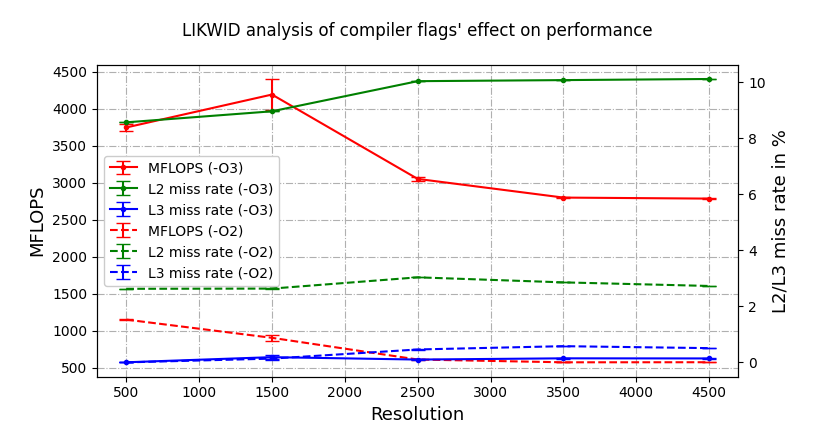
\includegraphics[scale=0.6]{figures/O2_vs_O3_forreport.png}
    \caption{MFLOPS, L2 and L3 miss rates of the compiler flag combinations -O2 and -O3 -fno-alias -xhost.}
    \label{fig:LIKWID}
\end{figure}

% check how the measurements are taken
The measurements show that while the higher compiler optimization flags achieve much better MFLOPS performance, they come with higher cache miss rates for the L2-level cache, and similar miss rates for the L3 cache. However, tables \ref{tab:profiling-O3} and \ref{tab:profiling-O2} show that the absolute numbers of cache misses are much lower for the higher compiler flags. This difference becomes especially dramatic when looking at the higher resolutions.

% table of cache misses in absolute numbers
\begin{table}[h]
\parbox{.45\linewidth}{
\caption{L2 and L3 misses for -O2.}
\label{tab:profiling-O2}
\begin{tabular}{|lll|}
\hline
%\multicolumn{3}{|l|}{-O2 performance}                                               \\ \hline
\multicolumn{1}{|l|}{Resolution} & \multicolumn{1}{l|}{L2 misses} & L3 misses \\ \hline
\multicolumn{1}{|l|}{500}        & \multicolumn{1}{l|}{6 623 795}   & 1244             \\ \hline
\multicolumn{1}{|l|}{1500}       & \multicolumn{1}{l|}{59 040 960}  & 4 746 497             \\ \hline
\multicolumn{1}{|l|}{2500}       & \multicolumn{1}{l|}{188 248 100} & 33 766 060             \\ \hline
\multicolumn{1}{|l|}{3500}       & \multicolumn{1}{l|}{347 108 400} & 83 620 390             \\ \hline
\multicolumn{1}{|l|}{4500}       & \multicolumn{1}{l|}{548 986 500} & 120 118 400             \\ \hline
\end{tabular}
}
\hfill
\parbox{.45\linewidth}{
        \caption{L2 and L3 misses for -O3 -fno-alias -xhost.}
\label{tab:profiling-O3}
\begin{tabular}{|lll|}
\hline
%\multicolumn{3}{|l|}{-O3 -fno-alias -xhost performance}                             \\ \hline
\multicolumn{1}{|l|}{Resolution} & \multicolumn{1}{l|}{L2 misses} & L3 misses       \\ \hline
\multicolumn{1}{|l|}{500}        & \multicolumn{1}{l|}{6 282 041}   & 1718             \\ \hline
\multicolumn{1}{|l|}{1500}       & \multicolumn{1}{l|}{56 318 080}  & 1 764 884             \\ \hline
\multicolumn{1}{|l|}{2500}       & \multicolumn{1}{l|}{156 413 500} & 1 933 281            \\ \hline
\multicolumn{1}{|l|}{3500}       & \multicolumn{1}{l|}{306 491 800} & 6 492 846              \\ \hline
\multicolumn{1}{|l|}{4500}       & \multicolumn{1}{l|}{506 600 600} & 9 072 937             \\ \hline
\end{tabular}
    }
\end{table}

Further investigating the performance with VTune gave more insight into how to improve the code's performance. The application was found to be back-end bound, with 67\% of of pipeline slots spent on memory operations. Moreover, hotspot analysis showed that 42\% of CPU time was spent on a copy operation. This is the operation at the end of the Jacobi relaxation where values from the newest iteration are copied into the old array. 

Based on these findings, the sequential program was optimized. The main speedup came from changing the memcpy operation to a pointer swap. In addition, the matrix access pattern was changed to align with C-style row-wise access, and the calculation of the residual was improved by combining its calculation loop with the loop of the relaxation step. This way, the stencil was only loaded to cache once instead of twice. The results of these changes are shown in figures \ref{fig:L2L3} and \ref{fig:runtimeL2L3}.

\begin{figure}[h]
    \centering
    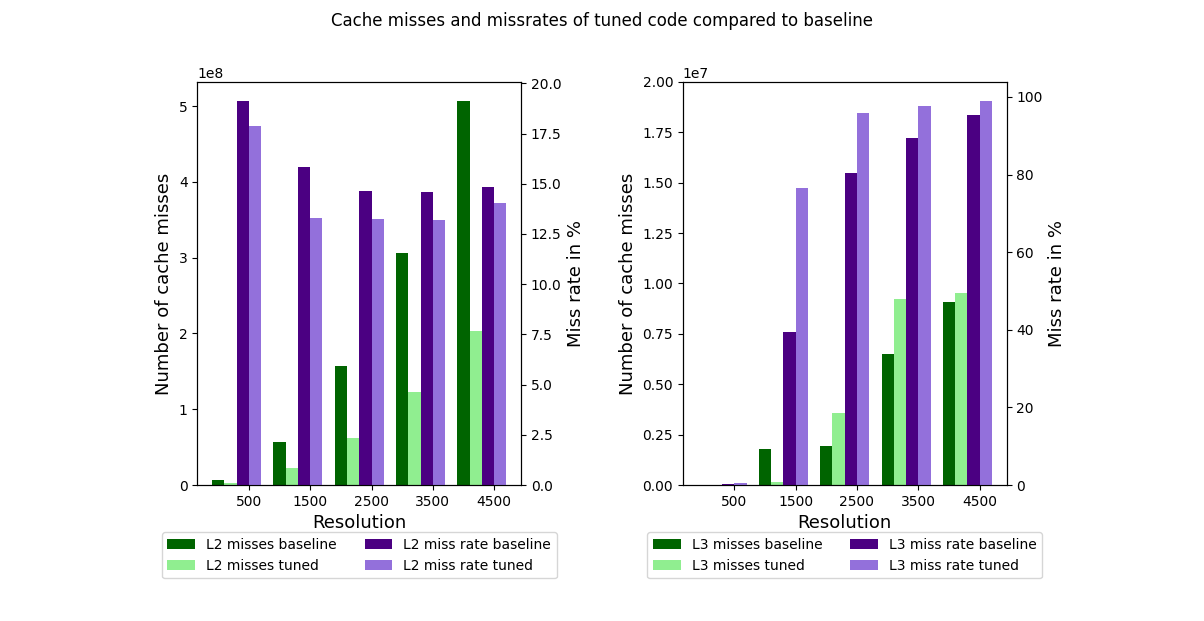
\includegraphics[scale=0.55]{figures/L2L3_and_rates.png}
    \caption{L2 and L3 cache misses and miss rates of the optimized code compared to the baseline.}
    \label{fig:L2L3}
\end{figure}

\begin{figure}[h]
    \centering
    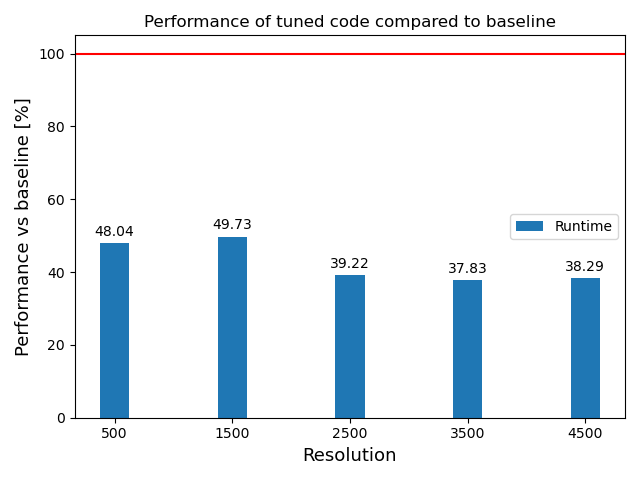
\includegraphics[scale=0.5]{figures/runtime_prof.png}
    \caption{Comparison of the runtime of the optimized code versus the baseline.}
    \label{fig:runtimeL2L3}
\end{figure}

From these results, it can be seen that the runtime of the code is significantly lower than before, down to only 40\% of the baseline. The L2 miss rates have also gone down, as well as the absolute numbers of L2 misses. However, it can be seen that the number of L3 misses has stayed at a similar order of magnitude, with worse performance for some resolutions. The L3 miss rates are between 95-98\% for the highest resolutions measured, implying that the changes made to the code still don't use the L3 cache effectively.




